\section{Geologic Map of Korea}
Hwang and colleagues \citeyearpar{hwang:2012} prepared a geo ontology model and geologic symbology using GIS representation of the digital geologic map units in Korea in order to develop Geological Information System for the geologic map of Korea using a spatiotemporal ontology model. 
Figure ~\ref{fig:petronto:geokorean} shows the onto
Geologic time was classified  with reference to the Korean geologic time scale defined by the Geologic Society in Korea, and to geologic dictionaries described in the previous section. 
~\ref{fig:petronto:geokorean2}
\begin{figure}[ht b]
  \begin{center}
    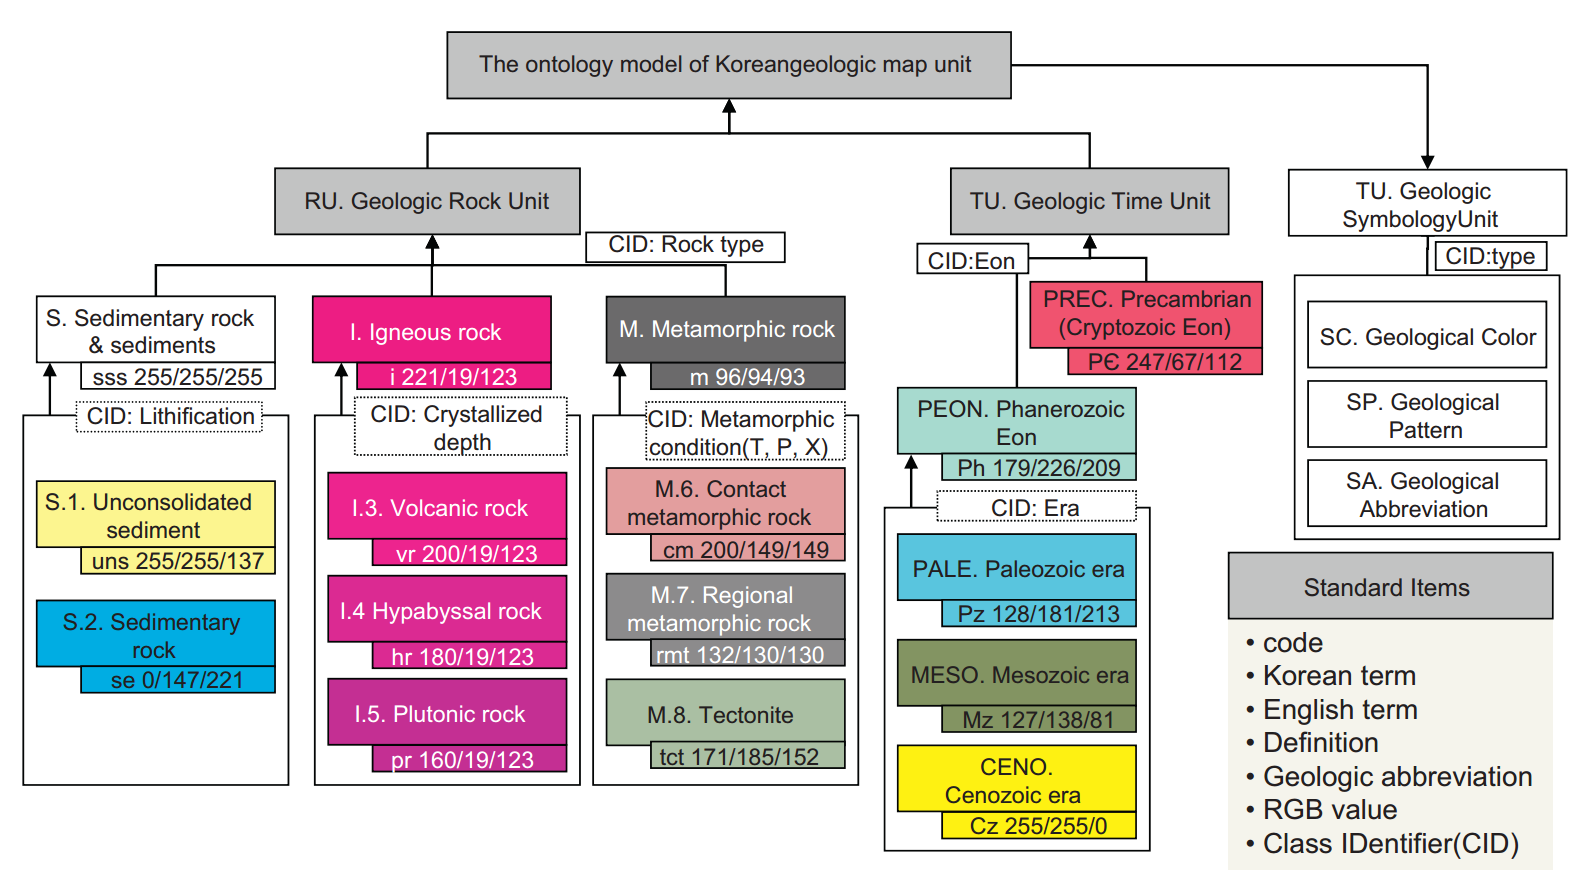
\includegraphics[width=1.0\linewidth]{ch-petro-onto/figures/geokorean}
    \caption{Ontology Model of the rock-time-simbology units~\cite{hwang:2012}}
    \label{fig:petronto:geokorean2}
  \end{center}
\end{figure}

\begin{figure}[p]
	\vspace*{2cm}    
    \makebox[\linewidth]{
		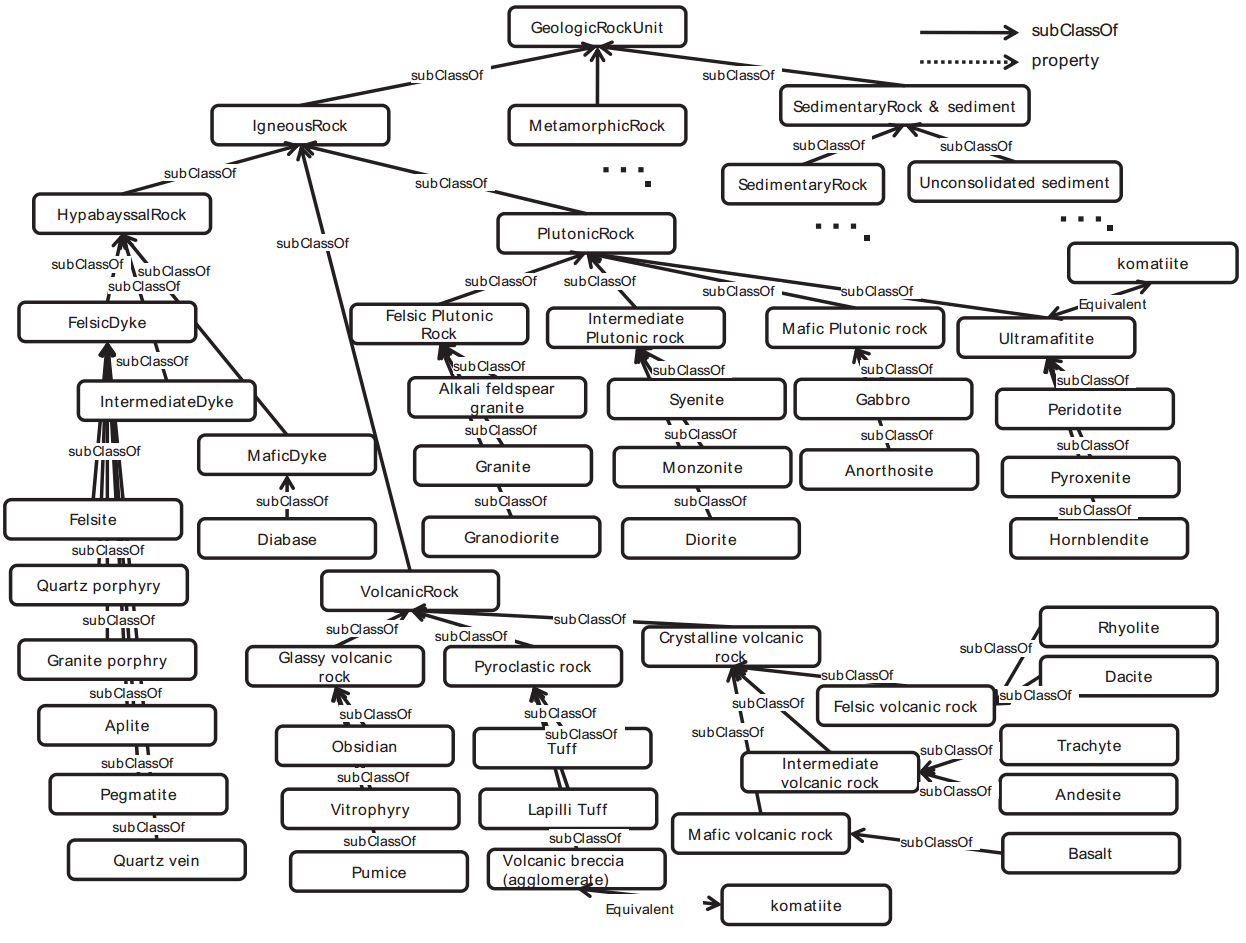
\includegraphics[width=1.3\linewidth,height=20cm]{ch-petro-onto/figures/geokorean2}
    }
     \caption{Ontology Model of the rock-time-simbology units~\cite{hwang:2012}}
     \label{fig:petronto:geokorean}
\end{figure}